\documentclass[12pt]{article}
\usepackage{mathtools}
\addtolength{\textheight}{.5in}
\addtolength{\textwidth}{1in}
\addtolength{\topmargin}{-.25in}
\addtolength{\evensidemargin}{-.5in}
\addtolength{\oddsidemargin}{-.5in}
\begin{document}

\title{$\Lambda$CDM and Modified Gravity: Descriptions of The Observed Universe at Different Cosmological Scales}
\author{Imran Hasan}
\date{December 2016}
\maketitle


Einstein's theory of gravity relates the curvature of spacetime to the stress energy tensor.

$$G_{\mu\nu} = R_{\mu \nu} - \frac{1}{2} g_{\mu \nu} R = 8\pi GT_{\mu \nu}$$

The theory has withstood several observational tests. Among them are Gravity Probe B's measurement of gravitomagnitism, and Eddington's measurement of the deflection of light by the sun. Additionally, GR is able to explain the advancement of the perihelion in Mercury's orbit, and recovers Newtonian gravity in the appropriate limits \cite{Caroll2004}. However, these tests occurred at length and mass scales no larger than those found in the solar system. On larger scales there is tension between the Einstein equations as described above, and astronomical and cosmological measurements \cite{Mavromatos2009}.

The canonical case study to see this is in the rotation curves of spiral galaxies. The measured rotational velocities of stars and gas is far higher than Einstein's gravity predicts, based on the content of luminous matter observed in these galaxies. One way to resolve the tension is to add non-baryonic forms of matter-energy to the Stress Energy Tensor. By adding a \emph{dark matter halo} to the density profile of spiral galaxies, we may recover the observed rotation curves. Another strategy is to alter the theory of gravity all together. The rotation curves may be recovered if we include correction terms to Newtonian gravity. One may view these perspectives as altering the right hand side of Einstein's equaiton for the former, and altering the left for the latter \cite{Bertone2004}. 

The previous example presents a boiler plate of how the remainder of the paper will follow. We will examine the abilities of dark matter/dark energy models and modified gravity models to explain observation, across different length and mass scales. To do this honestly, we must first define dark matter and dark energy, and discuss some theories of modified gravity. In the following three sections we discuss dark matter/dark energy in the $\Lambda$CDM cosmological model, and non-relativistic and relativistic models of modified gravity. Following the introductions to the theories, we investigate observational tests which show their strengths and weaknesses.

\section{$\Lambda$CDM}

Although there are several dark matter/dark energy models to choose from, one of the most tested and widely successful comes from $\Lambda$CDM cosmology, sometimes referred to as "standard cosmology". This paradigm can be understood by starting with the Friedmann Walkerson metric and Friedmann equations,

$$ds^{2} = -dt^{2} + a^{2}(t) (\frac{dr^{2}}{1 - kr^{2}} + r^{2}d\Omega^{2})$$

$$ H^{2} + \frac{k}{a^2} = \frac{8\pi G_{N}}{3} \rho_{tot}$$

where H is the Hubble Parameter, $\frac{\dot{a}(t)}{a(t)}$ \cite{Bertone2004}. In $\Lambda$CDM, we take k from the Friedmann metric and Friednmann equation to be zero, corresponding to a flat universe. From the Friedmann equation, we can see this leads to a restriction on the Stress Energy Tensor, $\rho_{c} = \frac{3H^2}{8\pi G}$. We then describe $\rho_{c}$ as being made up of different species,


$$\Omega_{i} = \frac{\rho_{i}}{\rho_{c}}$$

where 

$$\Omega = \sum_{i} \Omega_{i}$$

The different species are $\Omega_{M}$, $\Omega_{R}$, $\Omega_{\Lambda}$. $\Omega_{R}$, from radiation, is at a scale of ~$10^{-4}$, and thus the mass-energy budget is dominated by $\Omega_{M}$ and $\Omega_{\Lambda}$, matter and dark energy densities respectively \cite{Caroll2004}.

$\Omega_{M}$ and $\Omega_{\Lambda}$ have been measured by experiments like WMAP, SDSS, and Plank. The Plank measurement has the smallest error bars, and is consistent with the aforementioned experiments. It gives $\Omega_{M}$ = .308 $\pm$ 0.012  and $\Omega_{\Lambda}$  = 0.6911$\pm$ 0.0062 \cite{Plank2015}, \cite{SDSS2003}

$\Omega_{M}$ can be further subdivided into two categories, baryonic matter (the usual matter we encounter day to day, made up of protons and neutrons) and non-baryonic matter. Measurements of anisotropies in the cosmic microwave background , measurements of quasar spectra, and measurements of luminous mass in galaxy clusters puts $\Omega_{b}$ to be within 2-5 percent of $\rho_{c}$. This means the remaining matter in the universe is non-baryonic \cite{scott2002}.

Observational tests and numerical simulations have had some success in describing non-baryonic matter, or dark matter, as it is sometimes called. We defer a detailed description of dark matter until we address these experiments, their results, and implications for the $\Lambda$CDM paradigm later in the paper. However, for the time being it is worth briefly characterizing it. Dark matter is dynamically cold (hence the C in $\Lambda$CDM), in that it moves at speeds $<< $c. This means it will remain in close proximity to baryonic matter on galactic scales and higher, as it is unable to escape the gravitational potential of baryonic matter. It cannot interact with light, (hence dark), or if can, it does so very weakly. Furthermore, it is dissipativeless-it is unable to radiate light. And finally, It is collisionless \cite{Famaey2012}

Likewise, there have been successes in describing observations of the universe by invoking dark energy. We may take $\Omega_{\Lambda}$ to be the dark energy component of universe's mass-energy budget. This corresponds to an energy which pervades the universe and is responsible for its expansion \cite{scott2002}.

\section{Modified Theories of Gravity}

The earliest attempt to explain galactic-scale dynamics by changing Newton's laws of motion was offered by Milgrom in 1983. At large distances from galactic centers (at the kilo parsec scale), the accelerations of stars are on the order of $10^{-10}ms^{-2}$. He added an \emph{ad hoc} interpolating function that would connect the familiar acceleration regimes of newtonian gravity to these low order regimes via a smooth transition \cite{MilgromI1983}

$$ \mu (\frac{g}{a_{0}}) \mathbf{g} =\mathbf{ g_{N}} $$

where $a_{0}$ is a constant with units of acceleration, $\mu$ is the interpolating function, g is the true local accretion due to gravity, and $g_{N}$ is the newtonian acceleration obtained from Newton's inverse square law, $\frac{GM}{r^2}$. In order to stitch the two acceleration regimes in galaxies together, we require $\mu \rightarrow $ 1 as g $ >> a_{0}$, and $\mu(x) \rightarrow x$ for $x << 1$ \cite{Famaey2012}. A variety of 'families of $\mu$ functions' are discussed in the literature. However, we return to Milgrom's original discussion in 1983 to characterize it further, for the time being. By choosing $\mu(x) = x(1+x^{2})^{-2}$ and $a_{0}= 2 x 10^{-8} cms^{-2}$ the rotation curves of galaxies are recovered, with no need to add dark matter or any unseen matter \cite{MilgromII1983}.

We must pause here to emphasize Milgron's model is a \emph{new model of gravity altogether}. It is a departure from Newtonian gravity, and by extension cannot be captured by Einstein gravity in the weak field limit. By inspection of the functional form, it is clearly coordinate dependent, and not lorentz invariant. While Einstein's theory can follow from first principles by extremzing the Einstein-Hilbert action, Milgrom's modified gravity by itself is motivated primarily by observed data and has no analogous theoretical underpinnings. Nonetheless, Milgrom's description has had experimental successes and continues to do so in modern times. This has prompted theoretical work to develop a parent theory of Milgrom's modified gravity.

\section{Tensor Vector Scalar Gravity}
Tensor Vector Scalar theory of gravity has been proposed as an alternative to GR. TeVeS, as it is called, recovers GR, Newtonian gravity, and Milgrom's gravity. Additionally, it is relativistic, and motivated by a least action principle \cite{Bekenstein2004}. As the name suggests, it contains extra degrees of freedom in its action. A metric $\tilde{g}_{\mu \nu}$ with connection $\tilde{\nabla}$, a vector field, $A_{\mu}$, and a scalar field $\phi$. They are related in the following way

$$ g_{\mu \nu} = e^{-2 \phi} \tilde{g}_{\mu \nu} - 2\sinh (2\phi) A_{\mu} A_{\nu}$$

where $ g_{\mu \nu}$ is the metic in Einstein's GR \cite{Bekenstein2006}. $A_{\mu}$ obeys a normalization condition $A_{\mu} A^{\mu} = -1$ where $ A^{\mu} = \tilde{g}^{\mu \nu} A_{\nu}$ \cite{masud2014}. The action in TeVeS has additional components, due to these degrees of freedom.

$$ S = S_{\tilde{g}} + S_{A} + S_{\phi} + S_{m} $$

S is made up of the familiar Einstein-Hilbert action, a vector field action, scalar field action, and the familiar matter action, respectively. The new actions are defined as

$$ S_{A} = -\frac{1}{16G\pi} \int [K^{\alpha \beta \mu \nu} A_{\beta, \alpha} A_{\nu, \mu} - (\lambda/K)(g^{\mu \nu} A_{\mu} A_{\nu} + 1 )]  (-g)^{1/2} d^{4}x$$

where

$$ K^{\alpha \beta \mu \nu} = c_{1}\tilde{g}^{\alpha \mu} \tilde{g}^{\beta \nu}+ c_{2}\tilde{g}^{\alpha \beta} \tilde{g}^{\mu \nu} + c_{3}\tilde{g}^{\alpha \nu} \tilde{g}^{\beta \mu} + c_{4} A^{\alpha} A^{\mu} \tilde{g}^{\beta \nu}$$

with constants $c_{1}, c_{2}, c_{3}, c_{4}$. Spherically symmetric solutions depend only on $c_{1}$ and $ c_{4}$, incidentally. 
$$ S_{\phi} = -\frac{1}{2} \int [\sigma^{2}h^{\alpha \beta} \phi_{,\alpha} \phi_{,\beta} + \frac{1}{2} Gl^{-2} \sigma^{4}F(kG\sigma^{2})] (-g)^{1/2} d^{4}x$$

where $l$ is a scale parameter, F is an at the moment unspecified function, $\lambda$ is a lagrange multiplier filed which enforces normalization, $\sigma$ is a nondynamical scalar field, and finally $h^{\alpha \beta} = g^{\alpha \beta} - A^{\alpha} A^{\beta}$.  $F(kG\sigma^{2})$ is then chosen such that the correct nonrelativistic MONDian limit is obtained. Turning the crank and grinding through more math, we are presented with a new $\mu(y)$ function.\cite{Bekenstein2004}.

$$ -\mu F(\mu) -\frac{1}{2}\mu^{2} = y = kl^{2}(g^{\mu \nu} - A^{\mu}A^{\nu})\phi_{,\mu} \phi_{\nu}$$

$$ kG\sigma^{2} = \mu(kl^{2}(g^{\mu \nu} - A^{\mu}A^{\nu})\phi_{,\mu} \phi_{\nu})$$

At last, we discuss the limiting cases of TeVeS. As K $\rightarrow$ 0 and $l \rightarrow \infty$ GR is recovered \cite{Bekenstein2004}. In the weak limit the Newtonian potential $\Phi_{N}$, the scalar field $\phi$ and the potential $\Phi$ are related by 

$$\Phi = \Xi \Phi_{N} + \phi$$

where

$$\Xi = 1 + K/2 - 2\phi_{c} $$

where $K << 1$ is determined by the constants $c_{1}, c_{2}, c_{3}, c_{4}$, $\phi_{c} << 1$ the asymptotic limit of $\phi$, which is itself $<<$1. Thus, MOND + Newtonian gravity is recovered. The interpolating function offered by \cite{MilgromI1983} are found to be unphysical in TeVeS \cite{Angus2006}. Instead, \cite{Bekenstein2004} presents an interpolating function

$$ \mu(x) = \frac{2x}{1 + (2 - \alpha) + \sqrt{(1 - \alpha x)^{2} + 4x}}, 0 \leq \alpha \leq 1 $$

to make a toy model in the weak and intermediate gravity limit.

\section{Observational Tests of $\Lambda$CDM}
To evaluate the effectiveness of the dark matter/dark energy models, we will review some observational tests in the literature. In particular we will examine observations occurring at galactic scales and cluster scales. 

\subsection{galactic scales}

One of the earliest and most compelling cases for dark matter in galaxies comes from measuring the velocity of gas and stars in galaxies at different radii-the so called rotation curves mentioned earlier in the introduction. In these experiments, velocity measurements at different radii are taken by observing spectra of the galaxies. Using photometric measurements of the surfaces, mass to light ratios are constructed and used to model the mass  density in galaxy cores, and their disk components \cite{Bertone2004}. Assuming Newtonian gravity, the velocity of stars and gas in the galaxy can be predicted by using Poisson's equation. However, the predictions fall staggeringly short of capturing the true, measured velocity curves. If we insist on Newtonian gravity being the true weak limit of GR, than this implies an unseen mass distribution in galaxies which dominates the gravitational field near the edges \cite{Begeman1991}. Such measurements have first been made in the 1980's \cite{Knapp1987} and have continued to be made even in modern times \cite{Bertone2004}.
%figure for rotation curves 
\begin{figure}
\centering
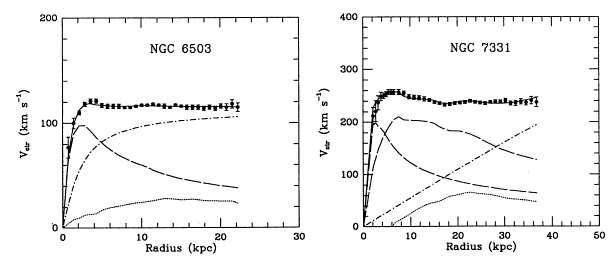
\includegraphics[width=5in]{darkMatterRotation.png}
\caption{rotation curves in two galaxies. Data with a reduced $\chi^{2 }$ best fit model are shown in points and solid line. Dashed dot lines for dark matter halo model, dashed lines for visible components, dotted lines for gas \cite{Begeman1991}}
\end{figure}
Alternative explanations to this so called \emph{hidden mass problem} which preserve Newtonian gravity and do not invoke an exotic new form of matter have been offered in the literature. In particular, rouge stellar mass black holes, neutron stars, white dwarfs in the milky way's halo would be sufficiently faint, considerably massive, and in the appropriate location in the Milky Way to explain its rotation curve. Observational surveys were carried out in the 90's to search for any evidence of these Massive Compact Halo Objects (MACHOs), but ultimately ruled them out \cite{Becker2005} \cite{Alcock2000}. Continuing microlensing projects that have lasted in modern times continue to rule these out, as well \cite{OGEL} \cite{MOA}.

The presence of dark matter has been implied in many other morphological varieties of galaxies, in addition to the spiral type galaxies discussed above. Different categories of Dwarf galaxies such as dwarf spheroidals, dwarf irregulars, ultra faint dwarf galaxies appear to be completely dominated by dark matter, upon investigation of their velocity dispersion and apparent brightness \cite{Simon2007}.

Taken all together, the dynamics of these various galaxies point to many of the tenets which $\Lambda$CDM insists upon. Requiring Newtonian gravity in the weak limit of Einstein's theory, we are confronted with a missing mass problem. The dynamical motions of matter in galaxies are too high to be explained by the luminous matter that can be detected. However, introducing a spherical distribution of unseen matter, which dominates in the density profile at large radii, can explain the observed dynamical properties. Observational surveys continue to rule out compact forms of baryonic matter as making up this unseen mass. This leaves us with a new form of matter, which interacts with gravity but not with light, and forms spherical halos around galaxies.

\subsection{cluster scales}
Cluster mergers offer an intriguing and fruitful theater to examine the predictions of $\Lambda$CDM. In Einstein's theory of gravity light follows geodesics, which are set by the curvature of space time. The geometry of space time is intern set by the stress energy tensor. This can lead to phenomena like the deflection of light, the Shapiro time delay, and gravitational lensing. By leveraging observations of gravitational lensing in clusters, we may in tern learn about the distribution of matter in those clusters. Whats more, we can use observations of these galaxies and compare the distribution of luminous matter to any matter that deflects but does not directly interact with light \cite{Caroll2004}.

%figure for bullet cluster
\begin{figure}
\centering
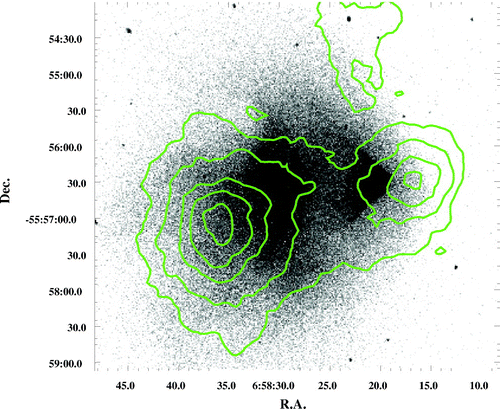
\includegraphics[height=3in]{bulletCluster.png}
\caption{bullet cluster X-ray imaging. Mass maps from weak lensing are show in the green contour overlays. There is a clear offset between the mass map centroids and X-ray-luminous gas \cite{Clowe2004}}
\end{figure}

The canonical example is the cluster 1E 065756, otherwise know as the \emph{Bullet Cluster}. 1E 065756 contains a bullet like sub-cluster passing through the main cluster, hence its colloquial name. In X-ray imaging, the gas of the sub-cluster-which has a bow shock and familiar collisional geometry-can be clearly identified. Using weak lensing of background galaxies, a mass map of the cluster can be created to identify the locations of gravity-interacting matter in the cluster. Astoundingly, the centroids of the weak lensing map and gas do not overlap, and are different at a 4-$\sigma$ confidence \cite{Clowe2004}. 

The weak lensing map is interpreted to outline the dark matter halos of the sub-cluster and clusters. Although the dark matter halos participate in gravity-creating the weak lensing effect-the dark matter itself is not visible in any wavelength. Additionally, the gas can be seen to lag behind the dark matter halos \cite{Clowe2004}. This is interpreted to mean the dark matter halos of the sub-cluster and cluster have not interacted with each other,  while the gas from the sub-cluster and cluster have participated in a collision-producing thermally excited gas and shock features. As a result, the bullet cluster provides evidence for unseen matter in galaxies which participates in gravity \emph{and} shows this dark matter is weakly interacting both in dark matter-dark matter interactions and dark matter-baryonic matter interactions \cite{Furlanetto2002}.

Other bullet cluster-like objects have since been discovered, which continue to enforce these properties of cold dark matter halos. Brade\v{c} et al. identified the cluster MACS J0025.4-1222, which consists of sub clusters which have passed through each other. Brade\v{c} again uses weak and strong lensing of background galaxy shapes to make a mass map, and X-ray imaging to detect the gas in the cluster. The centroids of the dark matter halos and gas are once more found to be off-set \cite{Bradec2008}.

Galaxy-galaxy interactions (specifically collisions and mergers) have made a very strong case for cold dark matter. With Einstein's gravity in hand, they show a distribution of collisionless but otherwise massive form of matter distributed around galaxies that is non-interacting with baryonic matter.  
%figure for marushas cluster which is like the bullet cluster
\begin{figure}
\centering
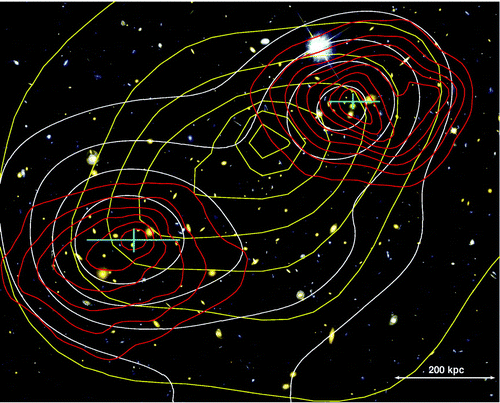
\includegraphics[height=3in]{marushaCluster.png}
\caption{color composite of MACS J00255.4-1222. Red contours show surface mass density from weak and strong lensing, yellow contours show X-ray brightness, and white contours show optical brightness. The dark matter halos are not spatially consistent with the X-ray or optical centroids\cite{Bradec2008}}
\end{figure}

\section{Observational tests of MOND and relativistic MOND}
While the theory has been debated (and criticized) heatedly in the literature, it must be pointed out that MOND has had some success in explaining phenomenology observed at different length scales. Indeed, some of the successes of $\Lambda$CDM are also offered in the MOND framework.  

\subsection{$ 10^{-10}$ ms$^{-2}$ scale experiments}
At the accelerations on the scale of $a_{0} \approx 10^{-10}$ms$^{-2}$, galactic dynamics in spiral galaxies deviate from the expected Newtonian result. The MOND framework accounts for this by describing accelerations at these scales by a non-Newtonian potential. As a result, experiments to detect departures from Newtonian motions at these regimes have been performed.

\cite{Gundlach2007} measure the force, acceleration, and angular position of a torsion pendulum in a carefully controlled laboratory setting. In the Newtonian limit the equations of motion are expected to follow from Hooke's law. In MOND the  $\mu$ function is expected to enforce a correction to the acceleration. One may write an MOND-like equation of motion for the pendulum as 

$$\tau(I,a,a_{0}) = \frac{Ia}{r} \mu(a/a_{0}) $$

Because of the plethora of $\mu$ functions offered in the literature, it is more tractable to treat the experiment as a null test, and look for departures from Newtonian dynamics, rather than look for a particular interpolating function. 

Accelerations as small of 5 X 10$^{-14}$ m/s$^{-2}$ in the torsion pendulum are measured by \cite{Gundlach2007}. The pendulum motion is well explained by Newtonian dynamics at this level-a full 4 orders of magnitude lower than $a_{0}$.

\begin{figure}
\centering
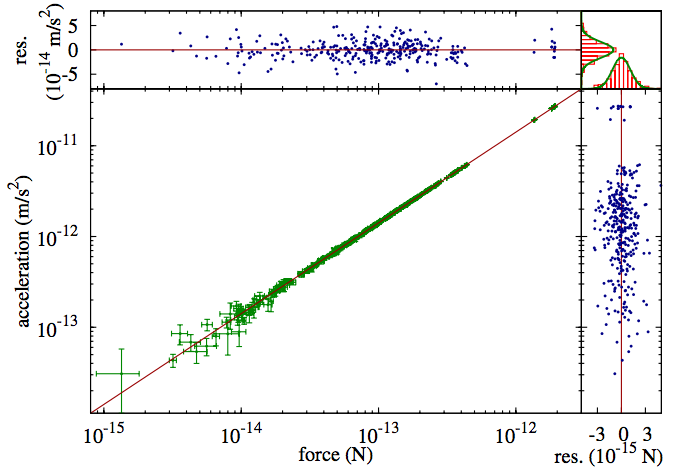
\includegraphics[height=3in]{pendulum.png}
\caption{Torsion pendulum force as a function of acceleration. The data are well explained by Hooke's law, even in the MOND regime of accelerations.  \cite{Gundlach2007}}
\end{figure}

It should be noted that this experiment does not rule out MOND and modified gravity. The setting of the experiment is systematically different, taking place in the presence of the Earth's gravitational potential on the Earth's surface, rather than a galactic potential at large radii. 
\subsection{galactic scale}
Predictions of galactic scale dynamics are one of MONDS strongest suits. Following from Milgrom's $\mu$ function and parameter $a_{0}$ described in section 2, galactic rotational velocities  can be fit well \cite{Begeman1991}. This has been one MONDs first, and enduring successes. From the MONDian perspective, it is not the mass content of galaxies which needs to be altered in order to explain rotation curves, but rather gravity itself. 

%figure for mond rotation curves
\begin{figure}
\centering
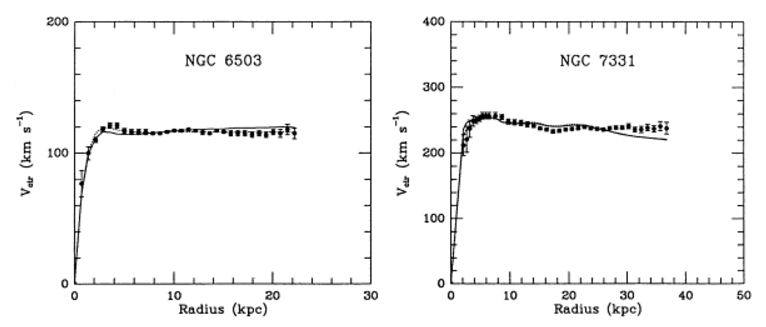
\includegraphics[width=5in]{mondRotation.png}
\caption{rotation curves in two galaxies. The data is fit with a MOND $\mu(x) = x(1+x^{2})^{-2}$ and selecting $x$ which reduces the $\chi^{2}$. Note these are the \emph{same two galaxies} as those in figure 1. MOND advocates often point out that MOND can explain rotational light curves just as well as dark mater models, and uses fewer degrees of freedom to do so. \cite{Begeman1991}}
\end{figure}

While classical dwarf galaxies are well described by MOND, the ultra faint dwarf galaxies described in the previous section (which are found to be dark matter dominated in $\Lambda$CDM models) are not well described by MOND. That is to say, MOND models are unable to fit the observed rotation curves of these objects \cite{Famaey2012}. 

On the other hand, tidal dwarf galaxies are well explained by MOND, and not explained well in the cold dark matter paradigm. Tidal dwarf galaxies are the result of the major merger of two spiral galaxies, whose resulting tidal tails create the tidal dwarf. In the CDM picture, the colissionless dark matter halos of the two spiral galaxies would have passed through each other, and the tidal dwarf is expected to have very little dark matter. As a result, there is no expected missing mass problem. Nonetheless, recent observations of three tidal dwarf galaxies show an apparent missing mass problem. Consequently, MOND fits can capture the rotation curve data, while CDM fits struggle \cite{Bournaud2007}. 

\begin{figure}
\centering
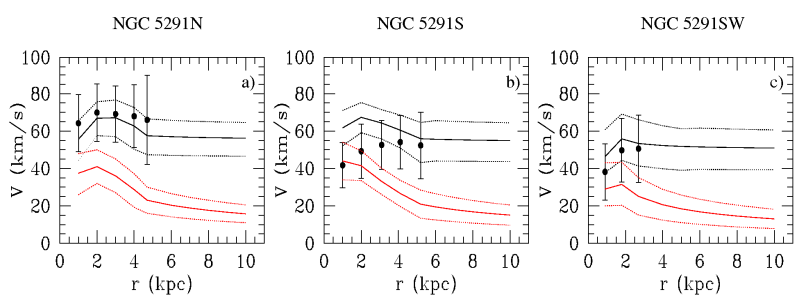
\includegraphics[width=6in]{tidalDwarf.png}
\caption{Rotation curves for three tidal dwarf galaxies. MOND fits are shown in black, CDM predictions in red. \cite{Bournaud2007}}
\end{figure}

Strong gravitational lensing fits into the relativistic TeVeS theory. In the weak limit, the calculation of deflection angles by light follows the calculation in a GR setting very closely. Instead of the Newtonian gravitational potential, the TeVeS weak limit is used as the lens potential. That is, use $\Phi = \Xi \Phi_{N} + \phi$ (described in section 3) instead of $\Phi_{N}$. Additionally, we must allow light to follow TeVeS geodesic equations, where $g_{\mu \nu} \mapsto \tilde{g_{\mu \nu}}, \nabla \mapsto \tilde{\nabla}$ \cite{Famaey2012}. 

Known strong lens galaxies have been explained in the TeVeS framework. In particular, \cite{Tian2013} was able to make measurements of the Hubble constant using time delay measurements of multiply imaged quasars, strongly lensed by spherical elliptical galaxies. Intriguingly, the value of $H_{0}$ is consistent with the result obtained by measurements of type Ia supernovae. 

However, for lens galaxies that are not spherical, success has been much less limited. \cite{Shan2008} successfully fits MOND density profiles to 11 non-spherical lens galaxies, which consequently accounts for the observed strong lensing of double and quadruply imaged quasars. On the other hand, \cite{Shan2008} were unable to explain strong lensing exhibited by 8 other non-spherically symmetric foreground galaxies in the weak TeVeS framework. \cite{Shan2008} and \cite{Famaey2012} posit that this is not an underlying failure of TeVeS in itself, but a short coming of the model fitting done by \cite{Shan2008}.

Overall, TeVeS has an inconsistent track record in explaining observed strong lens phenomena (\emph{sans} dark matter) when the foreground lens mass is at a galactic scale. It is able to use vanilla baryonic matter to account for the deflection angles of light rays coming from background quasars, as they are lensed by foreground spherical elliptical galaxies. \emph{On occasion} it can do this for asymmetric lens galaxies as well.

\subsection{cluster scales}
TeVeS lensing is less robust when the lens sources are galaxy clusters-the next rung up from galaxies on the cosmological mass ladder. \cite{Angus2006} simulates a mock bullet cluster like profile, whose potential is a linear combination of three off centered spherical weak limit TeVeS potentials. \cite{Angus2006} finds that TeVeS is able to create lensing and orbits which are consistent with those found in Newton-Einstein gravity. Based on the lensing model, matter density profiles can also be calculated using the TeVeS weak limit Poisson equation. However, the density profiles suggested \emph{do not} reflect the true underlying mass density in the lens plane. 

Other investigations in the literature show further weaknesses of MOND and TeVeS in this regime. Instead of using the weak limit, \cite{Mavromatos} numerically solves the full relativistic TeVeS equations of motion to calculate deflection angles, and do ray tracing for galaxy cluster lenses. These results are then used to calculate the mass in the galaxy cluster in the TeVeS framework. This procedure is followed for Einstein GR and weak limit MOND as well. The stellar mass of the galaxies, as calculated based on their photometries and colors, is compared to the TeVeS, GR, and MOND weak limit predictions.

In order to do the relativistic TeVeS calculation \cite{Mavromatos} needed to specify a $\mu$ function. The functions 

$$\mu(y) = \frac{\sqrt{y/3}}{1 - \frac{4\pi \alpha}{k} \sqrt{y/3}} $$
 
$$F(\mu) = \frac{6k^{3}}{(4\pi \alpha)\mu^{2}} [ln(\frac{4\pi \alpha \mu}{k} + 1)^{2} + \frac{1}{1 + \frac{4\pi \alpha \mu}{k}} - \frac{4\pi \alpha \mu}{k}]$$

are used, while for the MONDian weak limit, \cite{Bekenstein2004}'s $\mu$ function described at the end of section 3 is used

$$f(x)  = \frac{2x}{1 + (2 - \alpha) + \sqrt{(1 - \alpha x)^{2} + 4x}}$$

where $0 < \alpha \leq 1$. The TeVeS functions are chosen by \cite{Mavromatos} because the $\alpha = 0$ case corresponds to the weak limit, where the $\alpha = 1$ corresponds to the family of $\mu$ functions which best fits rotation curves of galaxies. f, F, and $\mu$ increase monatonically with $\alpha$, so the analysis can be confined between extreme values of $\alpha$.

Ultimately, the deflection angles calculated in all gravity scenarios were relatively consistent. However, the mass estimates for the lens clusters revealed a serious fault in TeVeS and MOND. The lens mass calculated by GR, MOND, and relativistic TeVeS were above the stellar mass of the lens clusters. For GR, this is predicted in the $\Lambda$CDM picture, the mass discrepancy is resolved by introducing dark matter halos. However, no such discrepancy is supposed to exist in the MOND or TeVeS picture. Indeed, the entire motivation of these theories was to alter gravity, so observed phenomena are explained by measured luminous mass. This shows that both MOND and TeVeS cannot simultaneously fit rotation curves and account for cluster scale lensing without adding dark matter \cite{Mavromatos}.

\begin{figure}
\centering
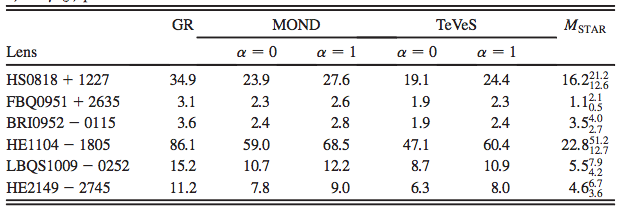
\includegraphics[width=6in]{tevesclustertab.png}
\caption{Baryonic mass of different lens clusters predicted by GR, MOND, and TeVeS. MOND and TeVeS exhibit the 'missing mass problem', requiring higher masses than those observed in the lens clusters from luminous matter. \cite{Mavromatos}}
\end{figure}


\begin{thebibliography}{99}
\bibitem{Alcock2000}Alcock C., et al., 2000, ApJ, 542, 281
\bibitem{Angus2006}Angus, G. W., Famaey, B., \& Zhao, H. S. 2006, MNRAS, 371, 138
\bibitem{Becker2005}Becker, A. C., et al. IAU Symp., 255, 357
\bibitem{Begeman1991} K. G. Begeman, A. H. Broeils and R. H. Sanders, 1991, MNRAS, 249, 523
\bibitem{Bekenstein2004} Bekenstein, J. D. 2004, Physical Review D, 70 
\bibitem{Bekenstein2006}Bekenstein, J. D.; Sanders, R. H., 2006, "A Primer to Relativistic MOND Theory", EAS Publications Series, 20: 225-230
\bibitem{Bertone2004} Particle Dark Matter: Evidence, Candidates, and Constraints. https://arxiv.org/abs/hep-ph/0404175
\bibitem{Bournaud2007}Bournaud, F. et al., 2007, Science, 316, 1166
\bibitem{Bradec2008}Brada\v{c} M., Allen S. W., Treu T., Ebeling H., Massey R., Morris R. G., von der Linden A., Applegate D., 2008, ApJ , 687, 959
\bibitem{Caroll2004}Carroll, Sean M. (2004), Spacetime and Geometry: An Introduction to General Relativity, San Francisco: Addison-Wesley, ISBN 0-8053-8732-3
\bibitem{masud2014}Chaichian, M., et al., 2014, Physics Letters B, 735, 322-326
\bibitem{Clowe2004}Clowe, D., et al., 2006, ApJ, 648, L109
\bibitem{scott2002} Dodelson, Scott (2008), Modern cosmology, San Diego, CA : Academic Press. ISBN 978-0122191411.
\bibitem{Famaey2012}Modified Newtonian Dynamics (MOND): Observational Phenomenology and Relativistic Extensions https://arxiv.org/abs/1112.3960
\bibitem{Furlanetto2002}Furlanetto, S. R., \& Loeb, A. 2002, ApJ, 565, 854
\bibitem{Gundlach2007}J. H. Gundlach et al., 2007, Phys. Rev Lett. 98, 150801
\bibitem{Knapp1987}Knapp, G. et al., 1987. Dark Mater in the Universe, IAU Symp. No. 117, Reidel, Dordrecht.
\bibitem{Plank2015} Collaboration, Planck; Ade, P. A. R.; Aghanim, N.; Arnaud, M.; Ashdown, M.; Aumont, J.; Baccigalupi, C.; Banday, A. J.; Barreiro, R. B.; Bartlett, J. G.; Bartolo, N.; Battaner, E.; Battye, R.; Benabed, K.; Benoit, A.; Benoit-Levy, A.; Bernard, J. -P.; Bersanelli, M.; Bielewicz, P.; Bonaldi, A.; Bonavera, L.; Bond, J. R.; Borrill, J.; Bouchet, F. R.; Boulanger, F.; Bucher, M.; Burigana, C.; Butler, R. C.; Calabrese, E.; et al. (2015). "Planck 2015 Results. XIII. Cosmological Parameters". arXiv:1502.01589
\bibitem{SDSS2003} K. N. Abazajian et al. 2009,  The Astrophysical Journal Supplement. 182, 543-558
\bibitem{Mavromatos2009}Mavromatos N. E., Sakellariadou, M., \& Yusaf, M. F, 2009, Phys. Rev. D 79, 081301(R)
\bibitem{MilgromI1983}  Milgrom, M.,  1983, AJ., 270, 365
\bibitem{MilgromII1983}  Milgrom, M., 1983, AJ., 270, 371-383
\bibitem{OGEL}OGLE Collaboration website. http://ogle.astrouw.edu.pl/
\bibitem{MOA}MOA Collaboration website. http://www.phys.canterbury.ac.nz/moa/
\bibitem{Shan2008}Shan, H.Y., Feix, M., Famaey, B. and Zhao, H.S., 2008, MNRAS, 387, 1303 - 1312,
\bibitem{Simon2007}Simon, Josh; Geha, Marla, 2007, AJ, 670, 1
\bibitem{skordis2011}Skordis, C. \& Zlosnik, T.G., 2011, Phys. Rev. D, 044044
(2008).
\bibitem{Tian2013}Yong Tian, Chung-Ming Ko, and Mu-Chen Chiu, 2013, AJ, 770, 2
\end{thebibliography}



\end{document}
